\documentclass[cjk,slidestop,compress,mathserif,blue]{beamer}
%\documentclass[cjk,slidestop,handout,compress,mathserif,blue]{beamer}	%打印PPT用,handout(讲义)可去掉过渡效果,如\pause引起的多页显示,为打印时节省纸张
%dvipdfm选项是关键,否则编译统统通不过
%beamer的颜色选项定义的是导航条和标题的颜色(即关键词structure的颜色)

%%%%%%%%%%%%%%%%仅限于XeTeX可使用的宏包%%%%%%%%%%%%%%%%%%%%%%%%%%%%
\usepackage{fontspec,xunicode,xltxtra,beamerthemesplit}
%\usepackage{beamerthemesplit}
\usepackage{handoutWithNotes}		%(讲义)在打印PPT的时候会留出给每一页做注释的部分
\usepackage{xeCJK}
\setCJKmainfont[BoldFont=黑体, ItalicFont=楷体, BoldItalicFont=仿宋]{黑体}
%\setsansfont[Mapping=tex-text]{Adobe 黑体 Std}
%如果装了Adobe Acrobat,可在font.conf中配置Adobe字体的路径以使用其中文字体
%也可直接使用系统中的中文字体如SimSun,SimHei,微软雅黑 等
%原来beamer用的字体是sans family;注意Mapping的大小写,不能写错

\usepackage{listings} 
\lstset{language=Matlab}%代码语言使用的是matlab 
\lstset{breaklines}%自动将长的代码行换行排版 
\lstset{extendedchars=false}%解决代码跨页时,章节标\dots

%%%%%%%%   确定标题和导航条结构的框架     %%%%%%%%%%%%
\usepackage{beamerthemeshadow}                       %
%\usepackage{beamerthemeclassic}%导航条色与背景色一致%
%%%%%%%%%%%%%%%%%%%%%%%%%%%%%%%%%%%%%%%%%%%%%%%%%%%%%%
\setbeamerfont{roman title}{size={}}
%\usepackage{CJK} % CJK 中文支持                                  %
\usepackage{amsmath,amsthm,amsfonts,amssymb,bm}
\usepackage{mathrsfs}
\usepackage{xcolor}                                        %使用默认允许使用颜色
\usepackage{hyperref} 
\usepackage{graphicx}
\usepackage{subfigure}           %图片跨页
\usepackage{animate}		 %插入动画
\usepackage{caption}
\captionsetup{font=footnotesize}

\usepackage{multirow}
% A LATEX package for embedding interactive Adobe Flash (SWF) and 3D files (Adobe U3D & PRC) as well as video and sound files or streams (FLV, MP4/H.246, MP3) into PDF documents with Adobe Reader-9
\usepackage[dvipdfmx]{movie15_dvipdfmx} %插入视频之一
%\usepackage{media9}			%插入视频之一
%\usepackage{multimedia}			%插入视频之一
%\usepackage{handoutWithNotes}		%(讲义)在打印PPT的时候会留出给每一页做注释的部分
%\pgfpagesuselayout{1 on 1 with notes landscape}[a4paper,border shrink=5mm]

%\usepackage[numbers,sort&compress]{natbib} %紧密排列             %
\usepackage[sectionbib]{chapterbib}        %每章节单独参考文献   %
\usepackage{hypernat}                                                                         %
\setbeamertemplate{bibliography item}[text] %参考文献前标注[]
%\usepackage[dvipdfm,bookmarksopen=true,pdfstartview=FitH,CJKbookmarks]{hyperref}		%
\hypersetup{bookmarksnumbered,colorlinks,linkcolor=brown,citecolor=blue,urlcolor=red}         %
%参考文献含有超链接引用时需要下列宏包,注意与natbib有冲突        %
%\usepackage[dvipdfm]{hyperref}                                  %
%\usepackage{hypernat}                                           %
\newcommand{\upcite}[1]{\hspace{0ex}\textsuperscript{\cite{#1}}} %

%\useoutertheme{smoothbars}
\useinnertheme[shadow=true]{rounded}
\usetheme{Berkeley}                                          %主题式样
%\usetheme{Luebeck}

\usecolortheme{lily}                                        %颜色主题式样

\usefonttheme{professionalfonts}                           %字体主题样式宏包

%\beamertemplatetransparentcoveredhigh                      %使所有被隐藏的文本高度透明
\beamertemplatetransparentcovereddynamicmedium             %使所有被隐藏的文本完全透明,动态,动态的范围很小
\mode<presentation>
%\beamersetaveragebackground{gray}                          %设置背景颜色(单一色) 
\beamertemplateshadingbackground{green!10}{red!5}         %设置背景颜色(渐变色)

%i放置单位logo
%\logo{
\includegraphics[width=1.6cm,height=0.35cm]{Figures/BCC_logo-1.png}}	%简单设置logo

%\pgfdeclareimage[width=3.5cm]{logoname}{Figures/BCC_logo-1.png}		%logo置于左侧微调
%\logo{\pgfuseimage{logoname}{\vspace{0.2cm}\hspace*{-2.0cm}}}

%在指定位置精确放置logo
\usepackage{tikz}
\usepackage{beamerfoils}
\usepackage{pgf}
%\logo{\pgfputat{\pgfxy(11.68,0.15)}{
\includegraphics[height=1.0cm,viewport=0 0 140 120,clip]{Figures/BCC_logo-1.png}}\pgfputat{\pgfxy(10.508,-0.22)}{
\includegraphics[height=0.369cm,viewport=140 0 540 120,clip]{Figures/BCC_logo-1.png}}}
%\MyLogo{
%	\pgfputat{\pgfxy(-50,-50)}{\pgfbox[right,base]{
\includegraphics[height=1cm]{Figures/BCC_logo-1.png}}}

%logo作为背景放置
%\setbeamertemplate{background}{
%	\pgfputat{\pgfxy(6.5,-0.5)}{\pgfbox[left,top]{\pgfimage[height=1.1cm]{Figures/BCC_logo-1.png}}}}

%\logo{}									%不显示logo

\begin{document}
%\begin{CJK*}{GBK}{song}
%\begin{CJK*}{GBK}{kai}
%beamer下不能用\songyi、\zihao等命令!
%\graphicspath{Figures/}

%-------------------------------PPT Title-------------------------------------
\title{京剧研究前辈“三大贤”}
%-----------------------------------------------------------------------------

%----------------------------Author & Date------------------------------------
\author[\textrm{Jun\_Jiang}]{枯石瘦木\inst{}
%\vskip -20pt 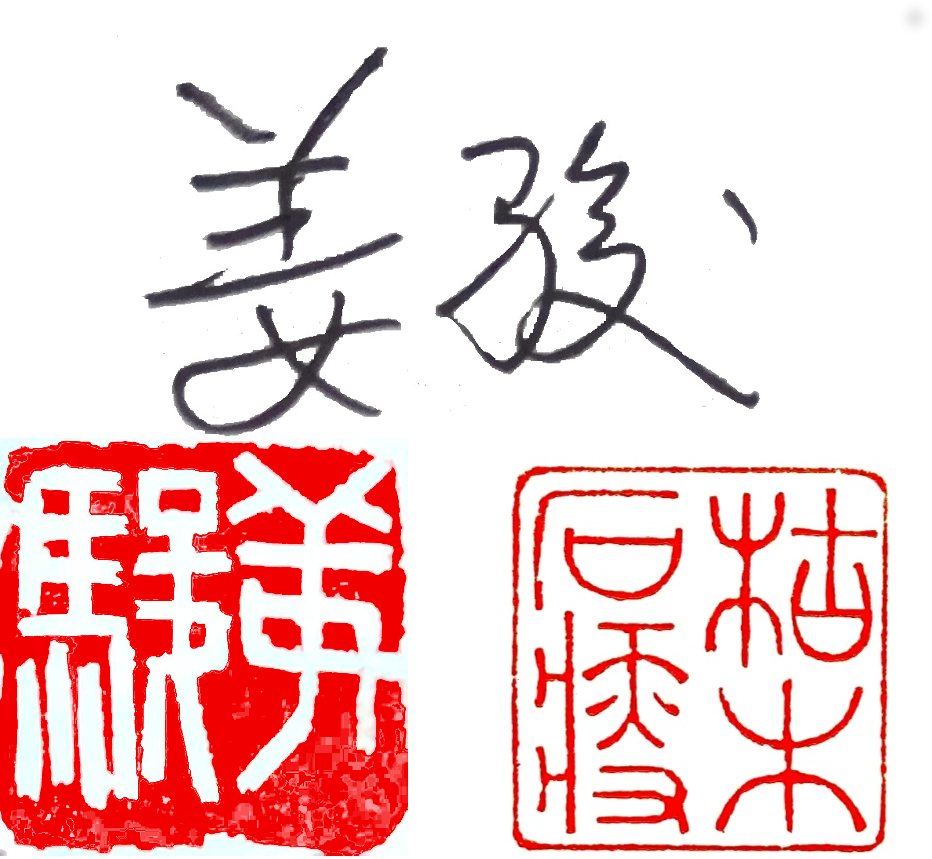
\includegraphics[scale=0.03]{Figures/signature-seal_Jiang-1.png} % 加入个人名章 
\vskip -20pt 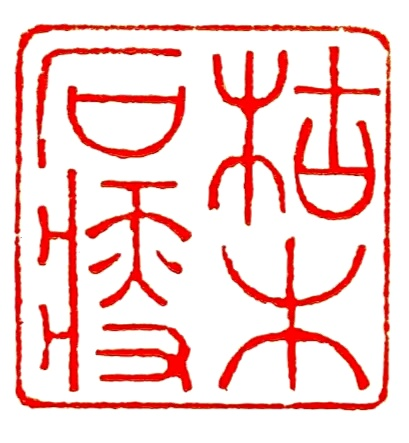
\includegraphics[scale=0.11]{Figures/seal_Jiang-2.jpg} % 加入个人名章 
} %[]{} (optional, use only with lots of authors)
% - Give the names in the same order as the appear in the paper.
% - Use the \inst{?} command only if the authors have different
%   affiliation.
%\institute[BCC]{\inst{}%
% \vskip -30pt 北京市计算中心}
\date[\today] % (optional, should be abbreviation of conference name)
{	{\fontsize{6.2pt}{4.2pt}\selectfont{\textcolor{blue}{E-mail:~}\url{czjiangjun@yeah.cn}}}
\vskip 10 pt {\fontsize{8.2pt}{6.2pt}\selectfont{报告地点   %清华大学\;\;物理系   
\vskip 5 pt \textrm{2018.09.29-30}}}
}

% - Either use conference name or its abbreviation
% - Not really information to the audience, more for people (including
%   yourself) who are reading the slides online

\subject{TEST-2}
% This is only inserted into the PDF information catalog. Can be left
% out.
\frame[allowframebreaks]
{
%	\frametitle{\fontsize{9.5pt}{5.2pt}\selectfont{\textcolor{orange}{“高通量并发式材料计算算法与软件”年度检查}}}
\titlepage
}
%-----------------------------------------------------------------------------

%------------------------------------------------------------------------------列出全文 outline ---------------------------------------------------------------------------------
\section*{}
\frame[allowframebreaks]
{
  \frametitle{Outline}
%  \frametitle{\textcolor{mycolor}{\secname}}
  \tableofcontents%[current,currentsection,currentsubsection]
}
%在每个section之前列出全部Outline
%类似的在每个subsection之前列出全部Outline是\AtBeginSubsection[]
\AtBeginSection[]
{
  \frame<handout:0>%[allowframebreaks]%讲义(handout)不显示 <handout:0> 讲义显示 <handout:1> / %beamer不显示 <beamer:0> beamer显示 <beamer:1>	
  {
    \frametitle{Outline}
%全部Outline中,本部分加亮
    \tableofcontents[current,currentsection]
  }
}

%------------------------------------------------------------------------------PPT main Body------------------------------------------------------------------------------------
\small
\section{“同光十三绝”}
\frame
{
	\frametitle{“同光十三绝”}
\begin{figure}[h!]
\centering
\vspace{-15.5pt}
\hspace*{-15.5pt}
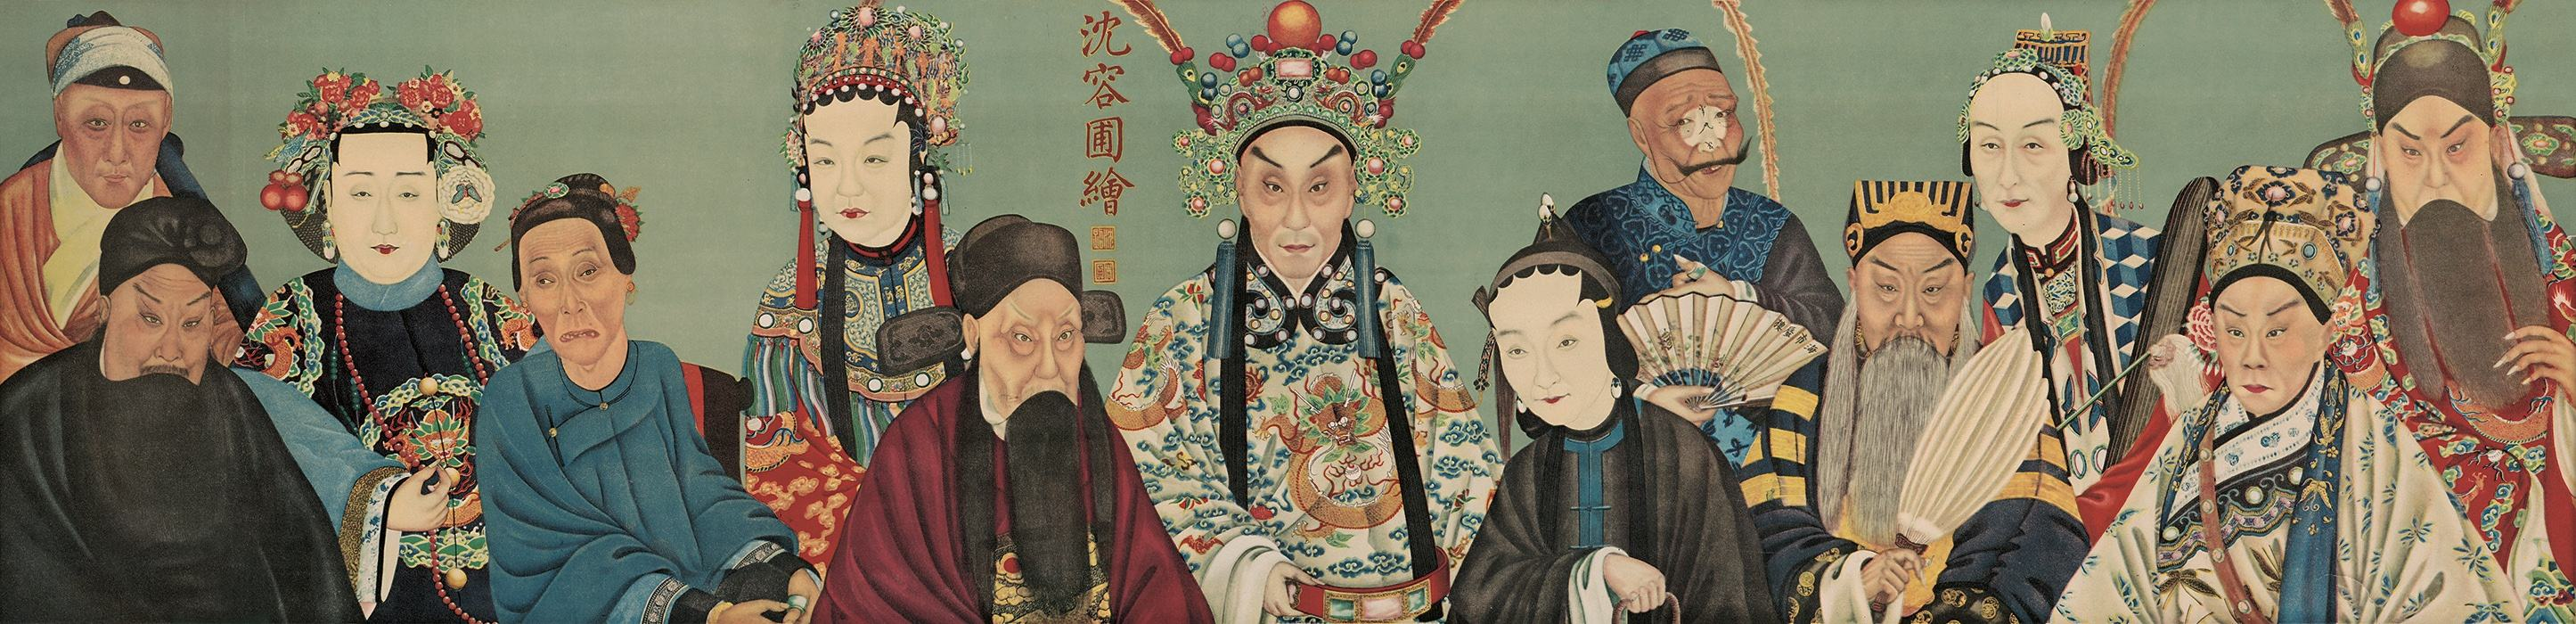
\includegraphics[height=0.26\textwidth,width=1.1\textwidth,viewport=0 0 2915 700,clip]{Figures/Tongguang_13-1.jpeg}
\caption{\fontsize{8.0pt}{6.2pt}\selectfont{\textrm{据传由晚清画师沈容圃绘制伶人戏装写真册页合成的“同光十三绝”画卷}}}
\label{Tongguang_13}
\end{figure}
\vspace{-5.5pt}
\fontsize{6.0pt}{3.9pt}\selectfont{\textrm{\textcolor{magenta}{左起:\qquad\;\;后排\qquad\qquad\qquad\qquad\qquad\qquad\qquad\qquad\qquad\;\;\;前排}\\
\qquad\qquad\;郝兰田(\textcolor{blue}{\!《行路训子》\!之\,康氏}) \qquad\qquad\;\;\;\;\;\;\;\;\;\;\;\;张胜奎(\textcolor{blue}{\!《一捧雪》\!之\,莫成}) \\
\qquad\qquad\;梅巧玲(\textcolor{blue}{\!《雁门关》\!之\,萧太后}) \qquad\qquad\;\;\;\;\;\;\;\;\;\;\;\;刘赶三(\textcolor{blue}{\!《探亲家》\!之\,乡下妈妈}) \\
\qquad\qquad\;余紫云(\textcolor{blue}{\!《彩楼配》\!之\,王宝钏}) \qquad\qquad\;\;\;\;\;\;\;\;\;\;\;\;程长庚(\textcolor{blue}{\!《群英会》\!之\,鲁肃}) \\
\qquad\qquad\;徐小香(\textcolor{blue}{\!《群英会》\!之\,周瑜}) \qquad\qquad\;\;\;\;\;\;\;\;\;\;\;\;\;\;\;\,时小福(\textcolor{blue}{\!《桑园会》\!之\,罗敷}) \\
\qquad\qquad\;杨鸣玉(\textcolor{blue}{\!《思志诚》\!之\,闵天亮}) \qquad\qquad\;\;\;\;\;\;\;\;\;\;\;\;卢胜奎(\textcolor{blue}{\!《战北原》\!之\,诸葛亮}) \\
\qquad\qquad\;朱莲芬(\textcolor{blue}{\!《玉簪记$\!\cdot\!$琴挑》\!之\,陈妙常}) \qquad\qquad\;\,谭鑫培(\textcolor{blue}{\!《恶虎村》\!之\,黄天霸}) \\
\qquad\qquad\;杨月楼(\textcolor{blue}{\!《四郎探母》\!之\,杨延辉})}}
}

\frame
{
	\frametitle{群英会}
\begin{figure}[h!]
\centering
\vspace{-0.2in}
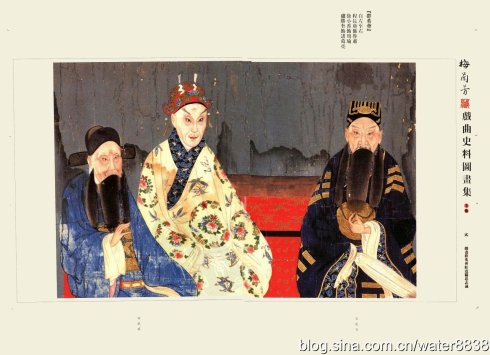
\includegraphics[height=0.55\textwidth,width=0.90\textwidth,viewport=39 41 313 221,clip]{Figures/Qunyinghui-2.jpeg}
\caption{程长庚、徐小香、卢胜奎合作《群英会》造像}
\label{Qunyinghui}
\end{figure}
}

\section{“三大贤”及其代表作}
\frame
{
	\frametitle{朱家溍先生}
\begin{figure}[h!]
\centering
\vspace{-0.2in}
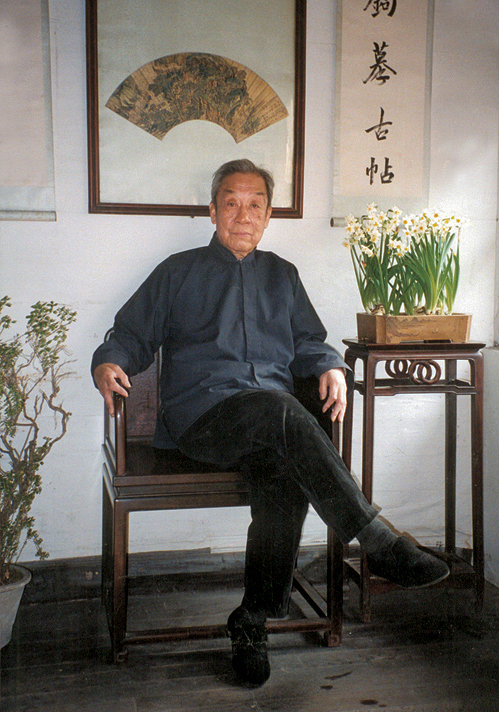
\includegraphics[height=0.64\textwidth,width=0.46\textwidth,viewport=0 0 500 720,clip]{Figures/Zhu_Jiajin.jpg}
\hskip 5pt
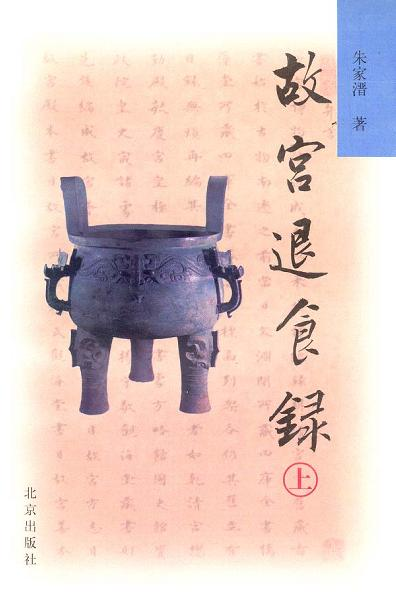
\includegraphics[height=0.64\textwidth,width=0.46\textwidth,viewport=0 0 450 610,clip]{Figures/Zhu_Tuishilu.jpg}
\caption{朱家溍先生(1914.8-2003.9.29)}
\label{Zhu_Jiajin}
\end{figure}
}

\frame
{
	\frametitle{刘曾复先生}
\begin{figure}[h!]
\centering
\vspace{-0.2in}
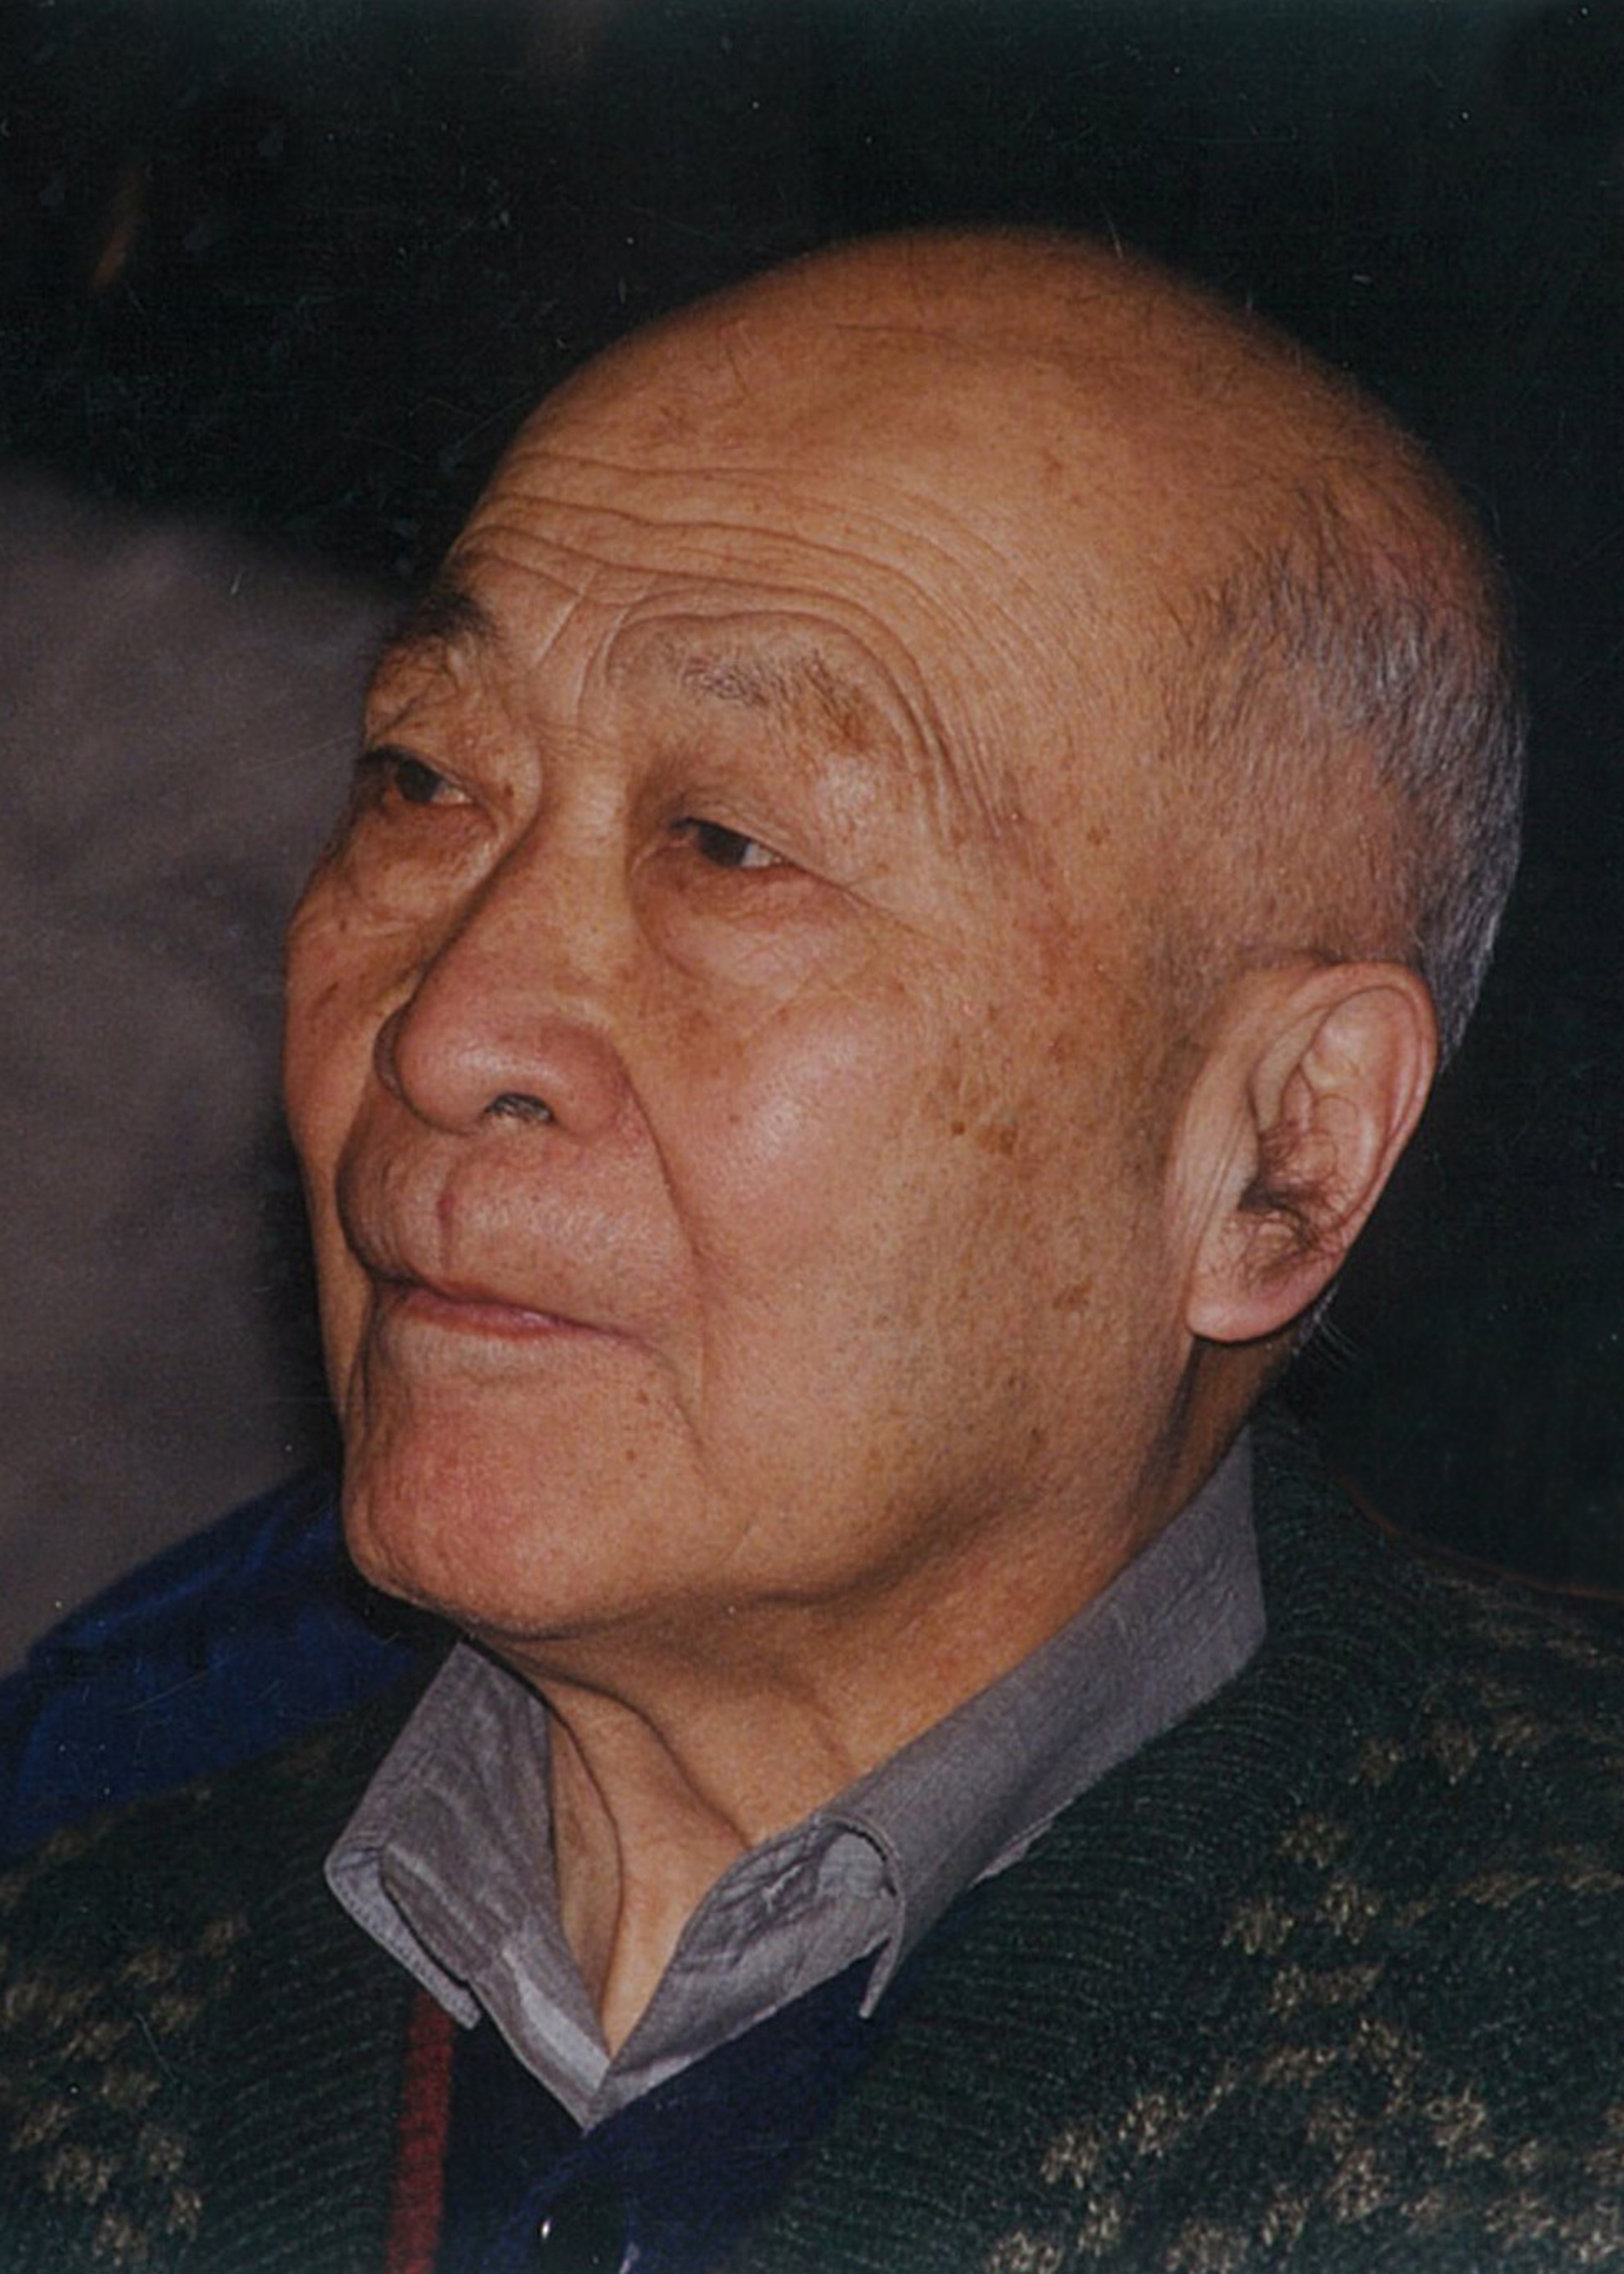
\includegraphics[height=0.64\textwidth,width=0.46\textwidth,viewport=0 0 360 520,clip]{Figures/Liu_Zengfu.jpg}
\hskip 5pt
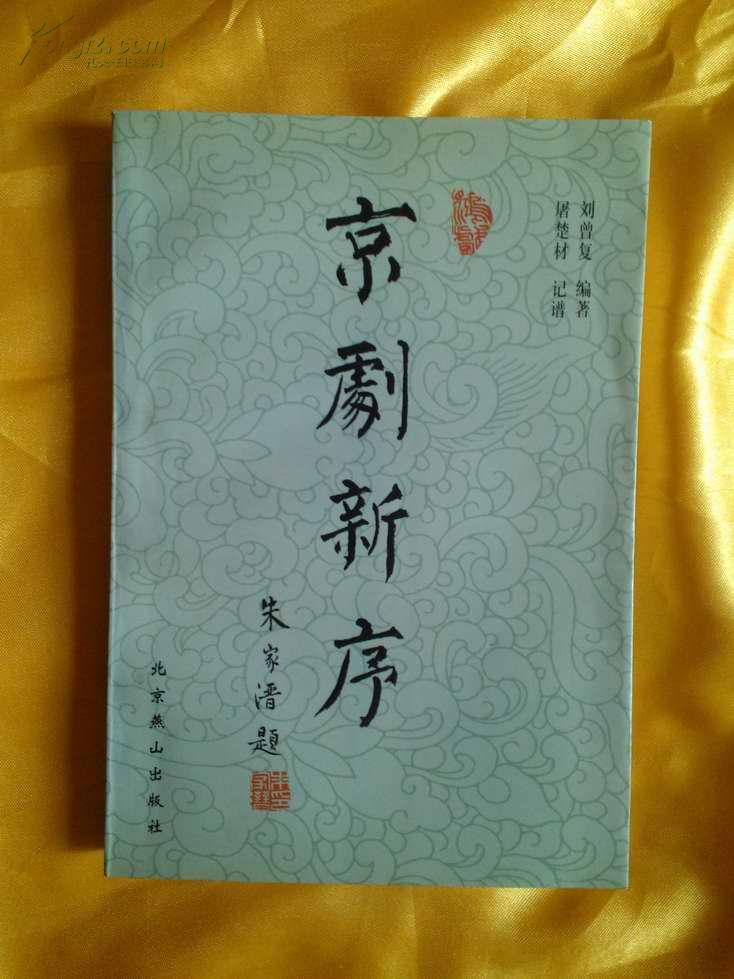
\includegraphics[height=0.62\textwidth,width=0.45\textwidth,viewport=100 85 660 875,clip]{Figures/Liu_Xinxu.jpg}
\caption{刘曾复先生(1914.11.9-2012.6.27)}
\label{Liu_Zengfu}
\end{figure}
}

\frame
{
	\frametitle{吴小如先生}
\begin{figure}[h!]
\centering
\vspace{-0.2in}
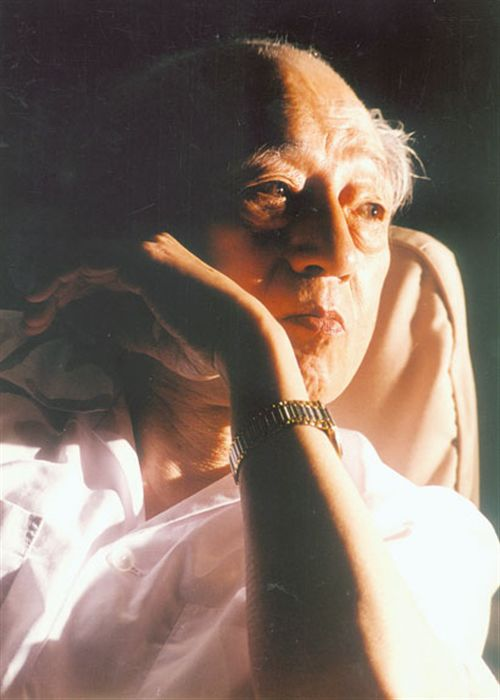
\includegraphics[height=0.64\textwidth,width=0.46\textwidth,viewport=0 0 360 520,clip]{Figures/Wu_Xiaoru.jpg}
\hskip 5pt
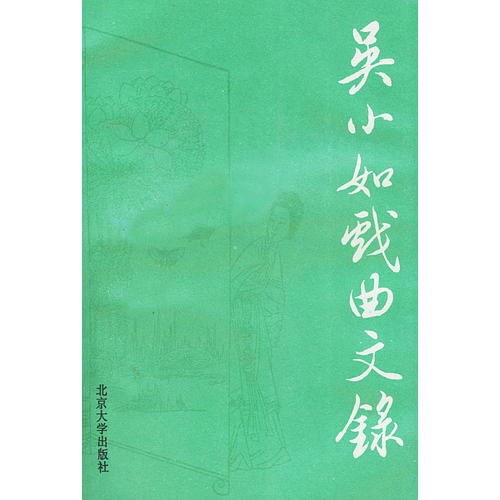
\includegraphics[height=0.64\textwidth,width=0.46\textwidth,viewport=39 5 200 235,clip]{Figures/Wu_Wenlu.jpg}
\caption{吴小如先生(1922.9.7-2014.5.11)}
\label{Wu_Xiaoru}
\end{figure}
}

\frame
{
	\frametitle{}
\begin{figure}[h!]
\centering
\vspace{-10.5pt}
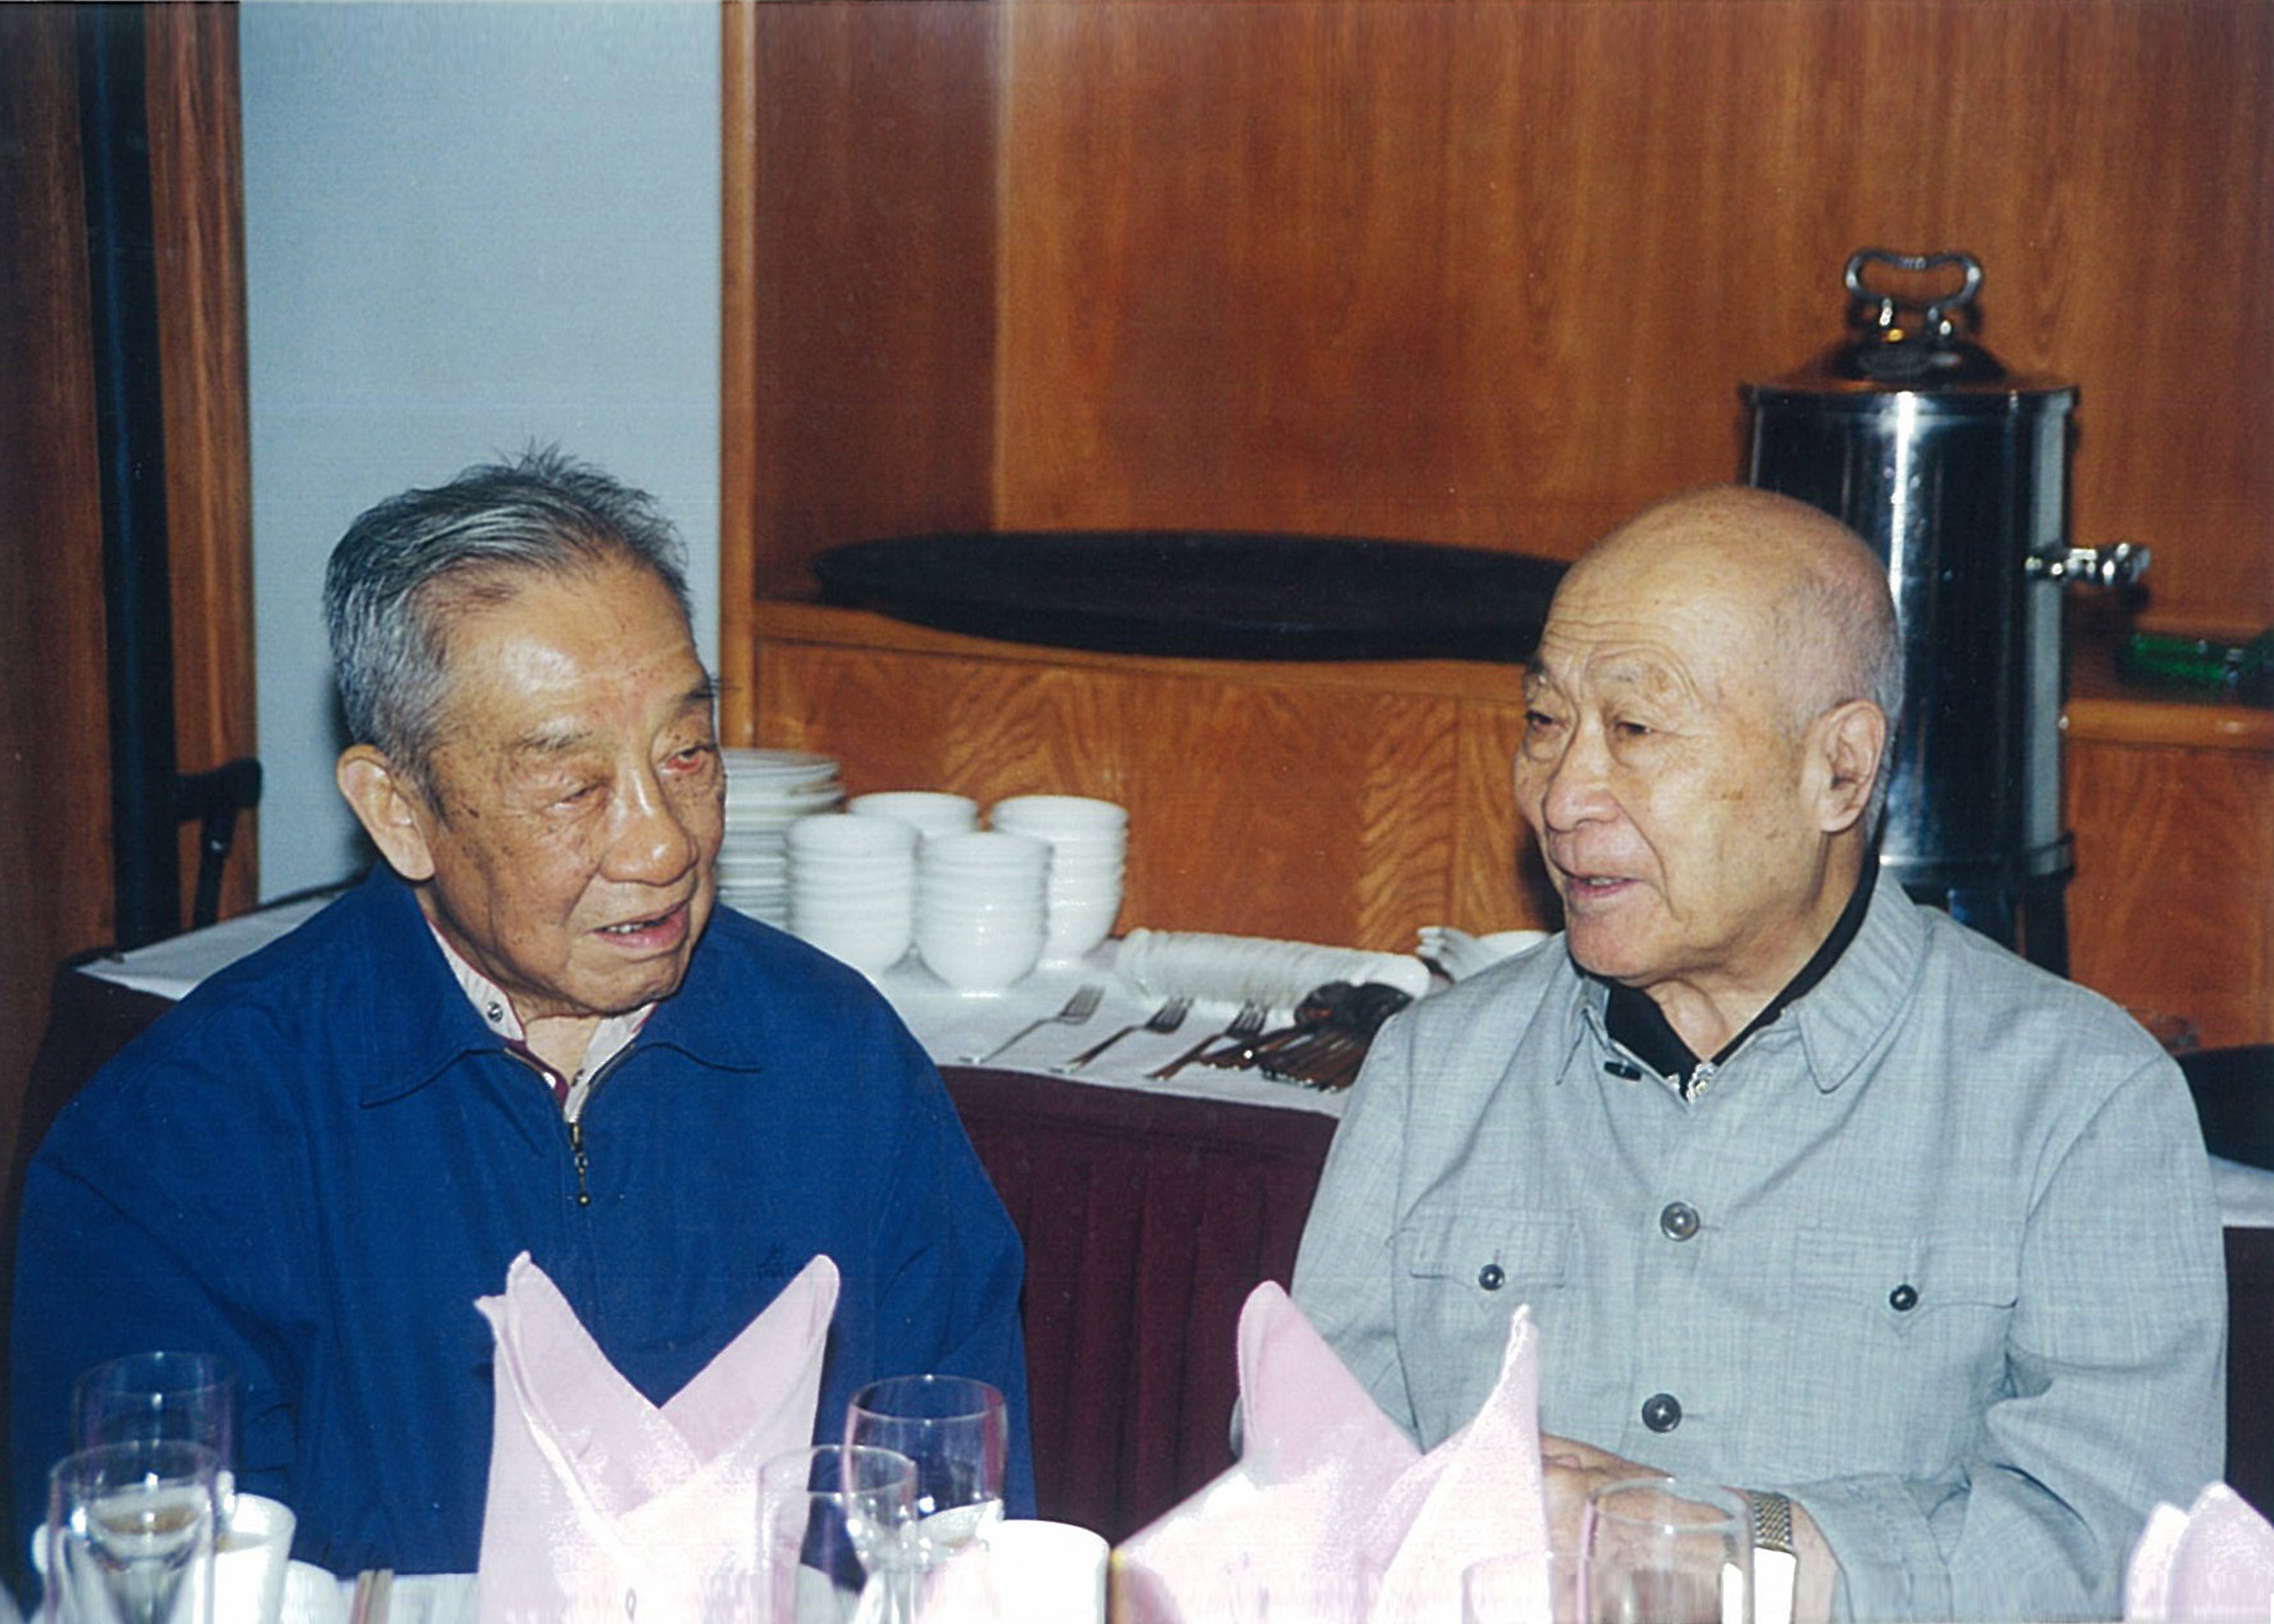
\includegraphics[height=0.60\textwidth,width=0.9\textwidth,viewport=0 0 510 350,clip]{Figures/Zhu-Liu.jpg}
\caption{\textrm{朱家溍先生与刘曾复先生合影}}
\label{Collect_Zhu-Liu}
\end{figure}
}

\frame
{
	\frametitle{}
\begin{figure}[h!]
\centering
%\vspace{-10.5pt}
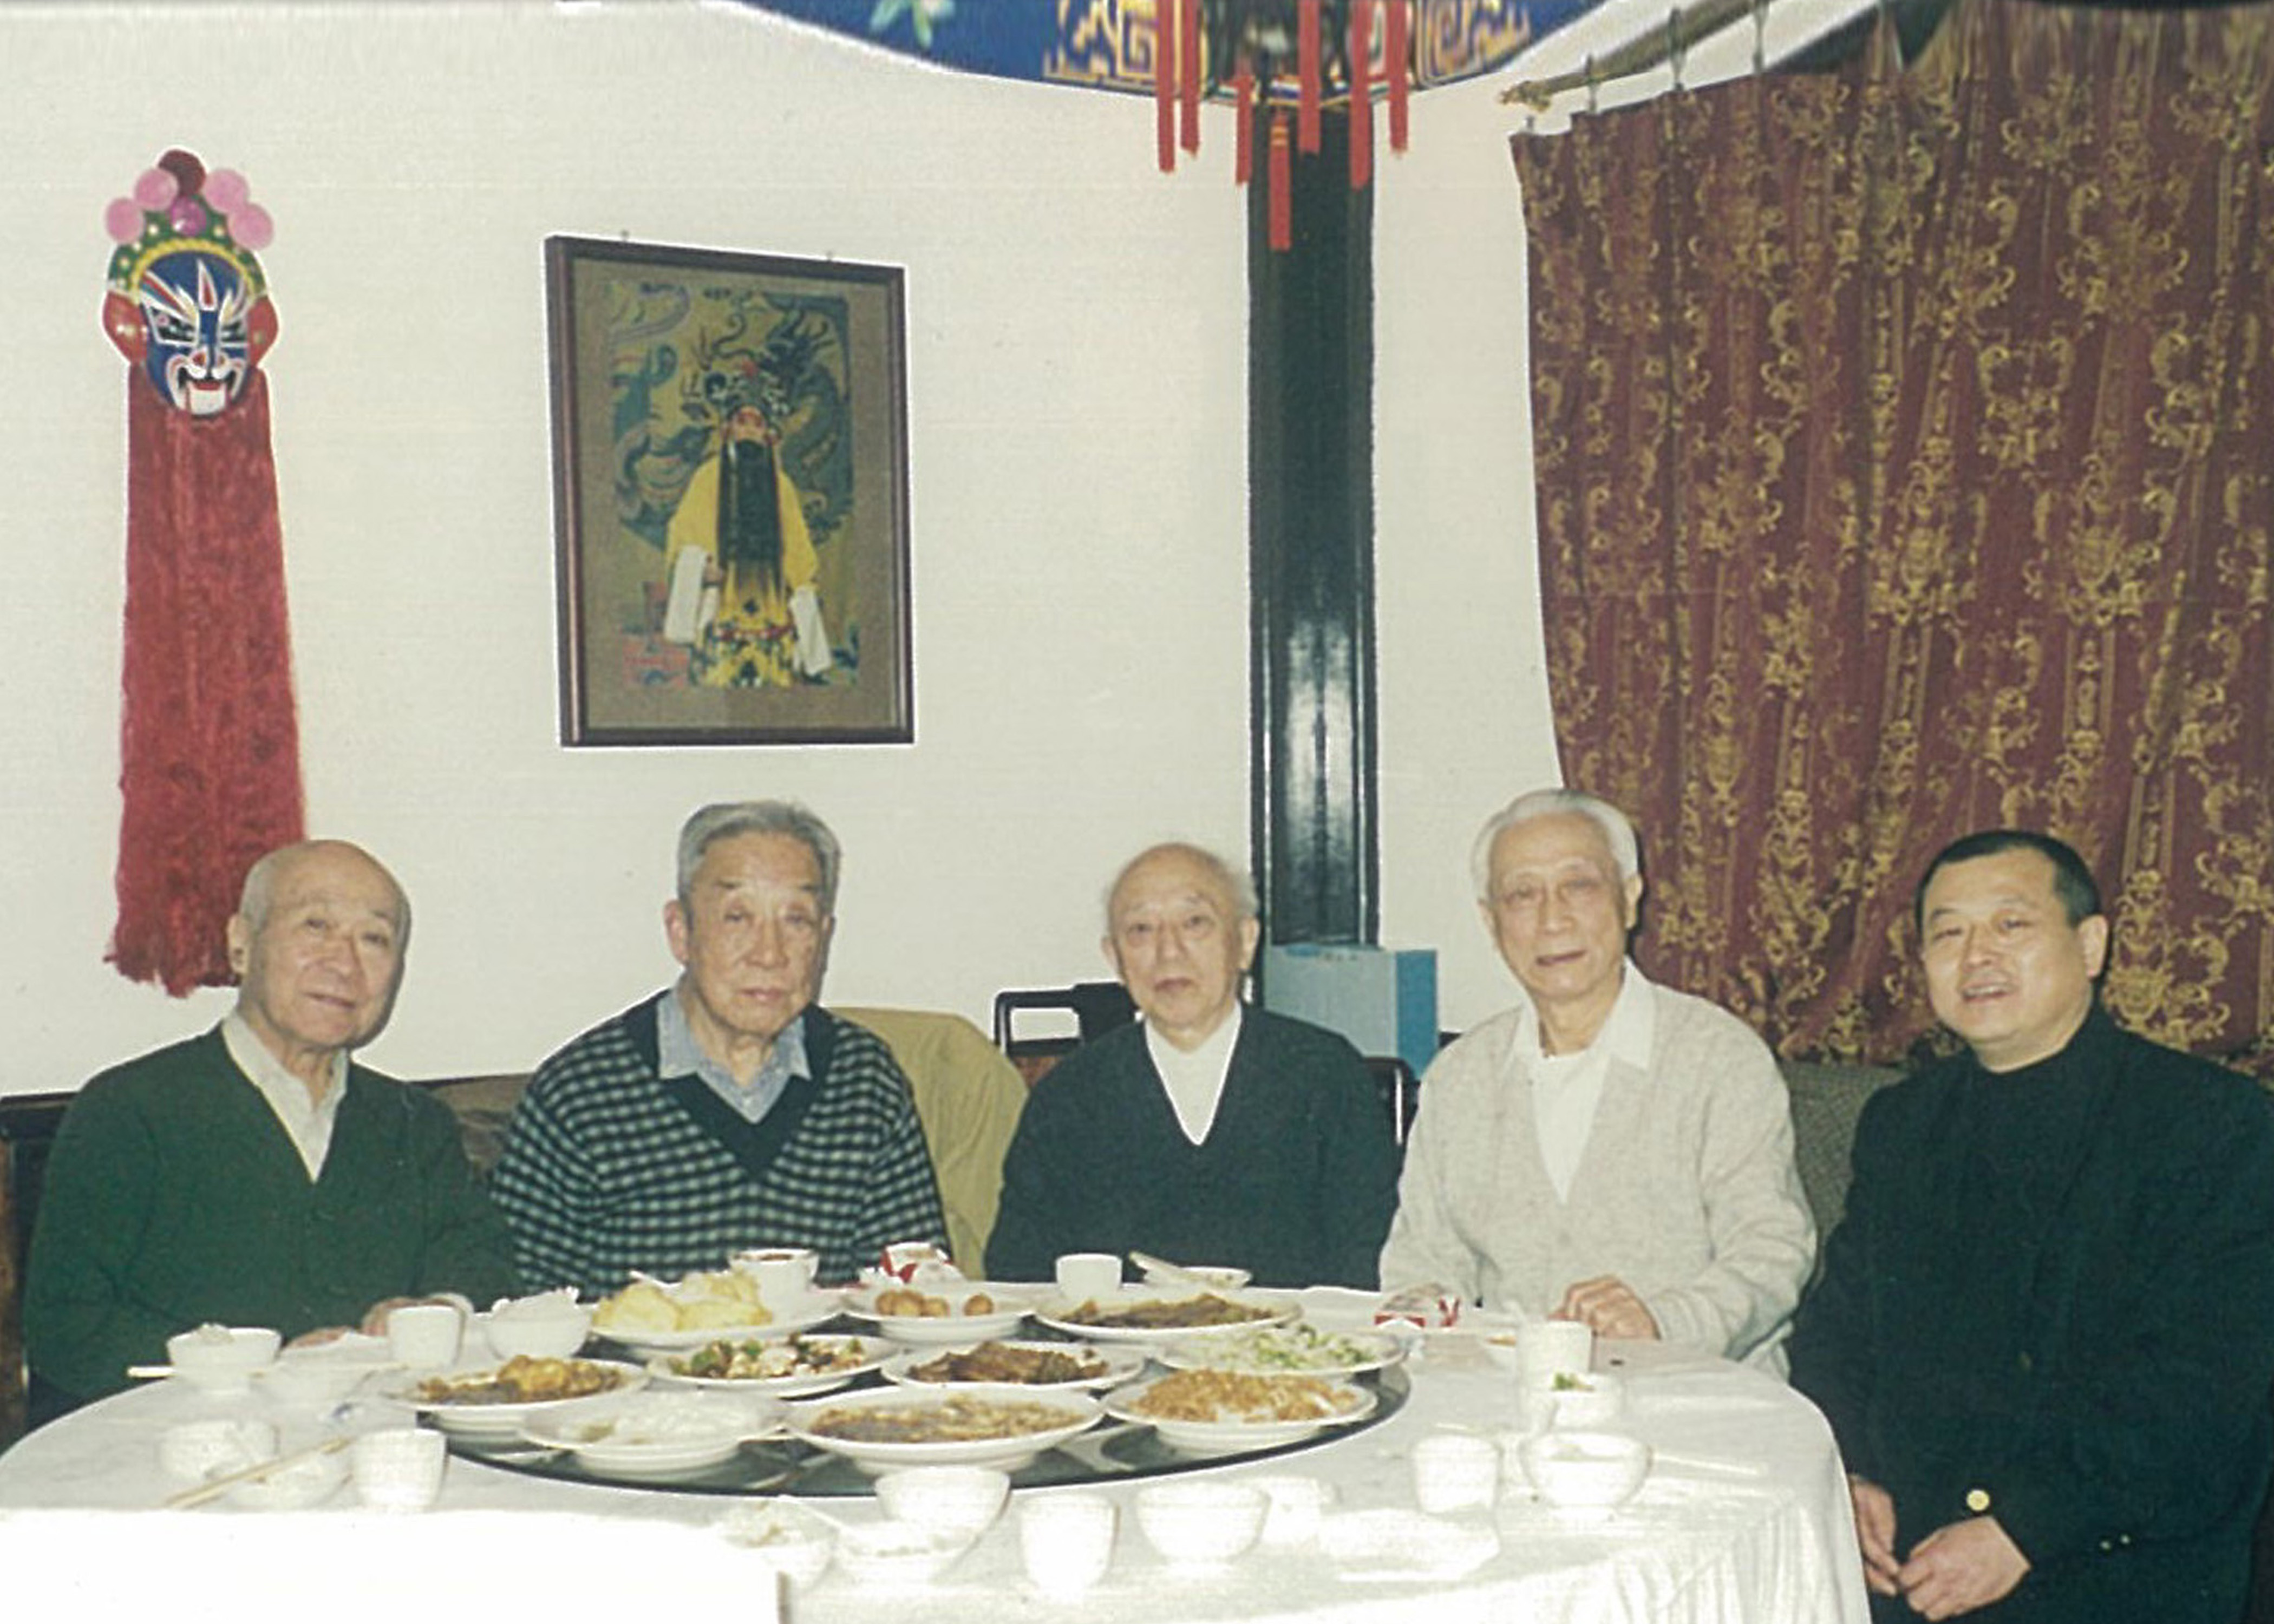
\includegraphics[height=0.60\textwidth,width=1.0\textwidth,viewport=0 0 500 300,clip]{Figures/Collect_Zhu-Liu-Wu-Wang.jpg}
\caption{\fontsize{7.3pt}{3.9pt}\selectfont{\textrm{左起:~刘曾先生、朱家溍先生、吴小如先生、王金璐先生(1919-2016.6.1)等合影}}}
\label{Collect_Wang}
\end{figure}
}

%\frame
%{
%	\frametitle{答辩合影}
%\begin{figure}[h!]
%\centering
%\vspace{-10.5pt}
%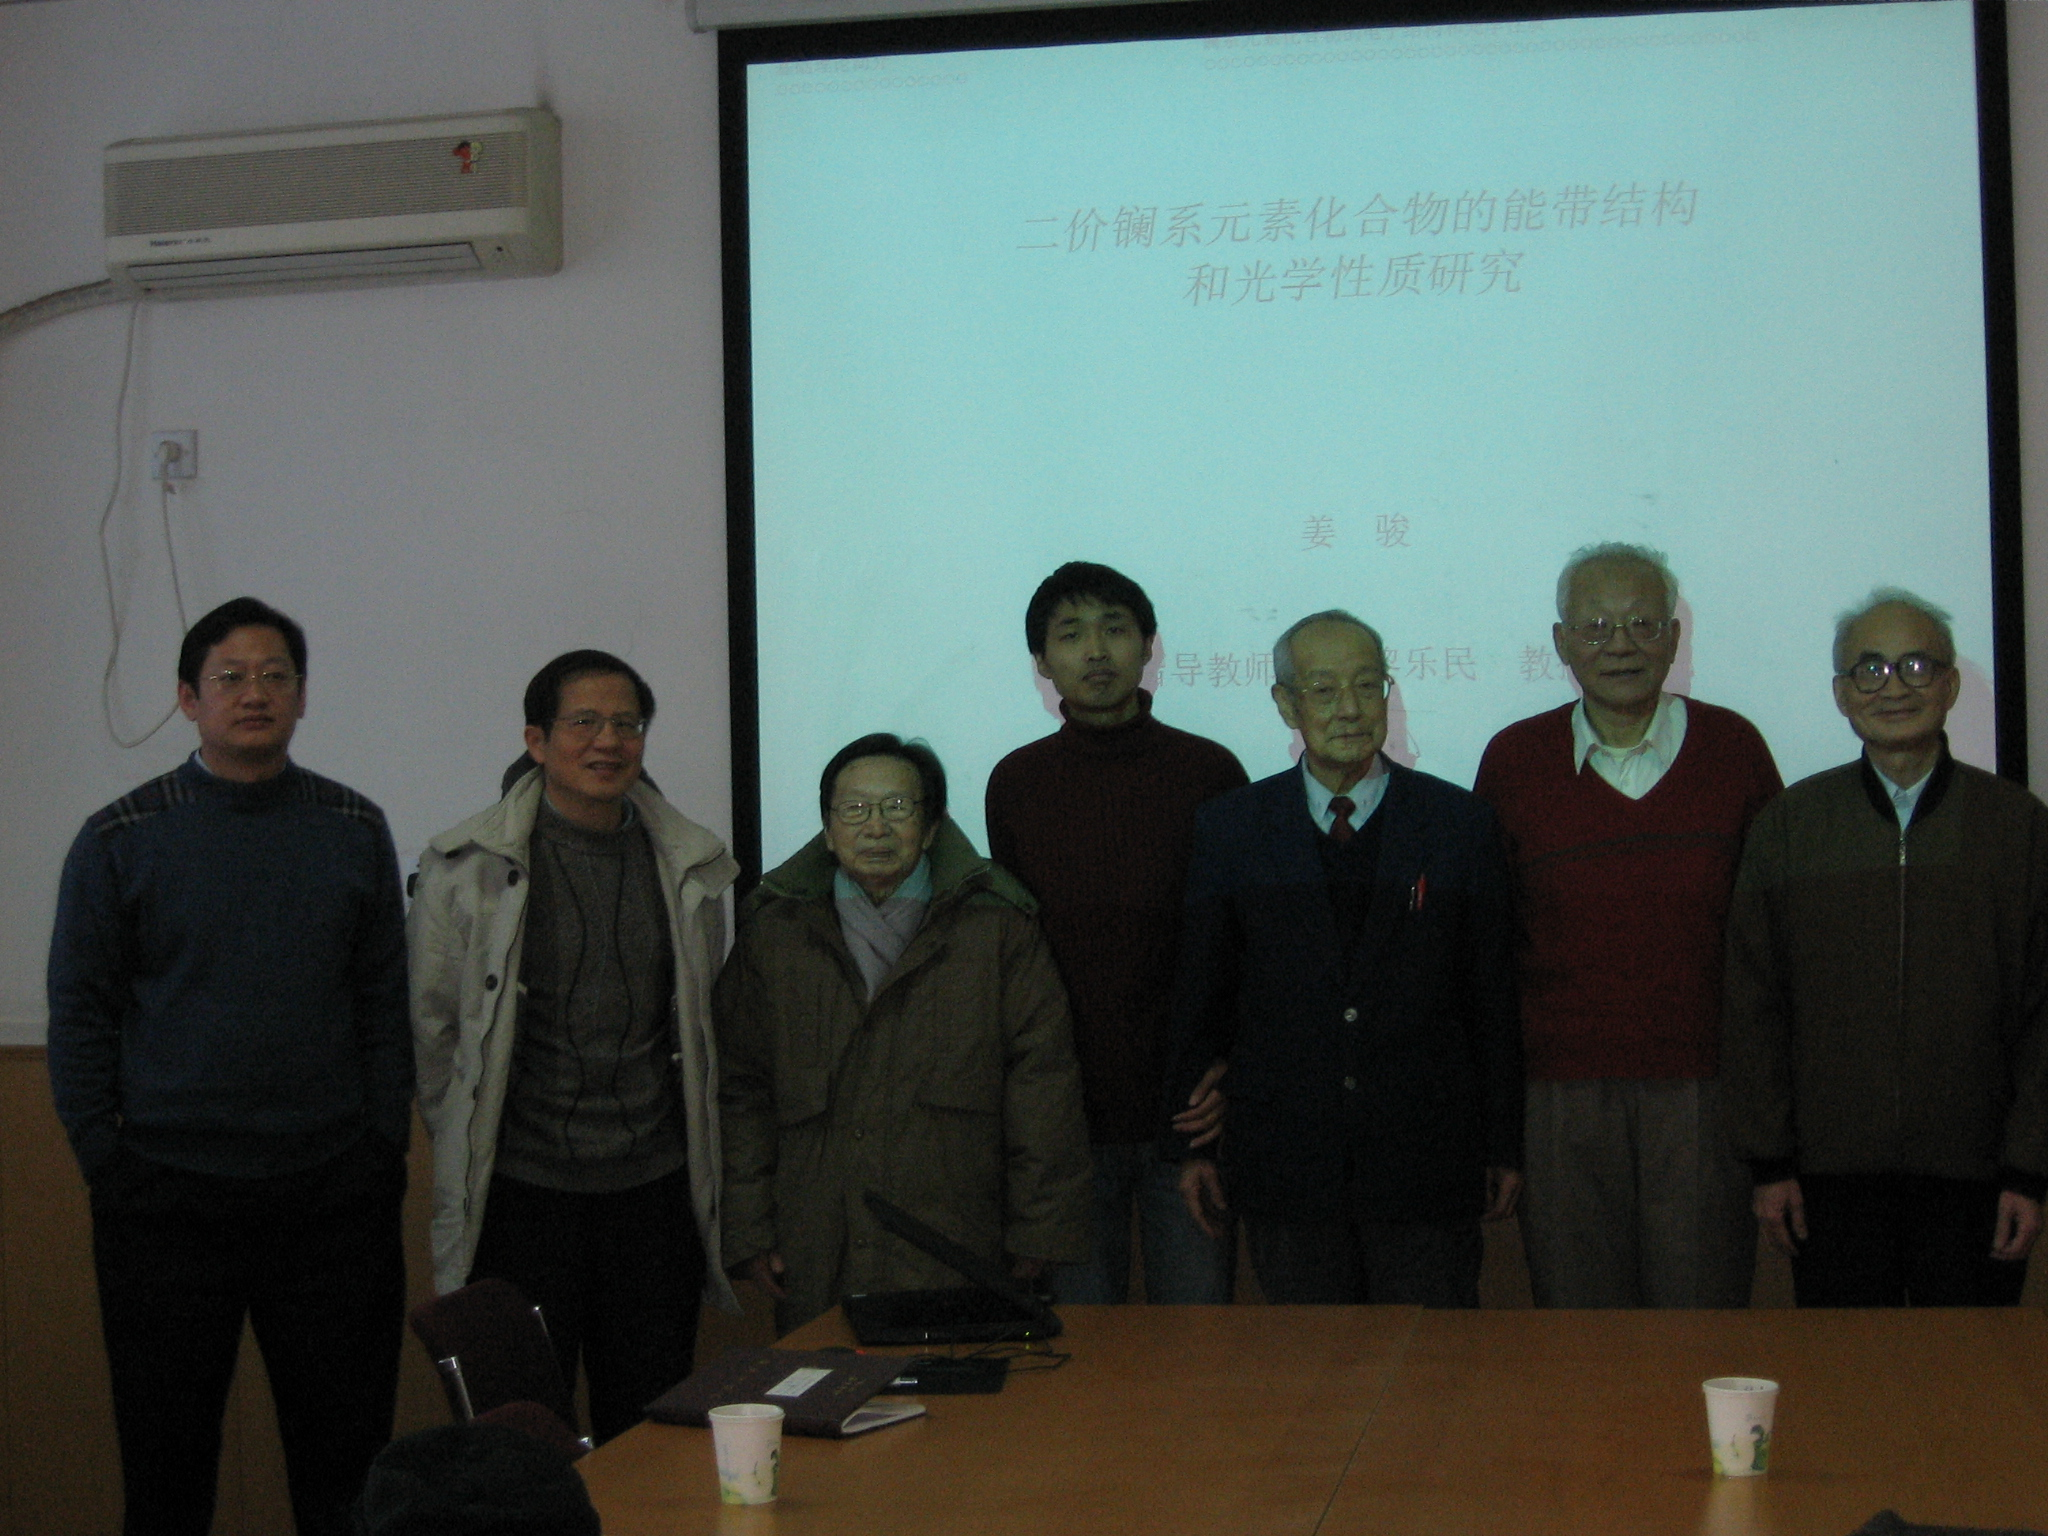
\includegraphics[height=0.62\textwidth,width=0.9\textwidth,viewport=0 0 820 600,clip]{Figures/Thesis_Defense_2007.jpg}
%\caption{\textrm{2007.12.15博士论文答辩后留影:}\\{\fontsize{7.1pt}{3.9pt}\selectfont\textrm{左起:~刘文剑教授、黄元河教授、刘若庄教授、答辩人、徐光宪教授、王德民教授、黎乐民教授}}}
%\label{Thesis_Defense_2007}
%\end{figure}
%}

%%%%%%%%%%%%%%%%%%%%%%%%%%%%%%%%%  插入音频/视频,使用url 要求视频在指定目录下 %%%%%%%%%%%%%%%%%%%%%%%%%%%%%%%%
%%%%%%%%%%%%%%%%%%%%%%%%%%%%%%%%%%%%%%%%%%%%%%%%%%%%%%%%%%%%%%%%%%%%%%%%%%%%%%%%%%%%%%%%%%%%%%%%%%%%%%%%%%%%%%%
\frame<handout:0>										 	      %
{													      %
	\frametitle{京剧名宿遗音}									      %
\begin{figure}[ht]											      %
%	\includemovie[poster, autostart,controls, mouse, url, text=(xx), repeat] {0.8\textwidth}{0.6\textwidth}{traffic.avi}		      %
%	\includemovie[poster, controls, mouse, url] {0.8\textwidth}{0.6\textwidth}{traffic.avi}		      %
	%\includemovie[poster, controls, mouse, url] {0.8\textwidth}{0.6\textwidth}{Yuan_Kuocheng.mp4}	      %
	\includemovie[poster, controls, mouse, url] {0.8\textwidth}{0.2\textwidth}{Figures/Liu-Xiongzhouguan.mp3}     %
	\includemovie[poster, controls, mouse, url] {0.8\textwidth}{0.2\textwidth}{Figures/Zhu_Liu-Luomahu.mp3}	      %
%	\includemovie[poster, controls, mouse, url] {0.8\textwidth}{0.2\textwidth}{Figures/Liu-Pantaohui.mp3}	      %
	\includemovie[poster, autostart, mouse, url, repeat] {0.8\textwidth}{0.2\textwidth}{Figures/Wu-Pantaohui.mp3}	      %
\caption{京剧名宿遗留音}											      %
\end{figure}												      %
}

%\begin{frame}
%	\frametitle{frame with sound}
%\dots
%\includemedia[ 
%	label=my_sound,
%	width=1ex, height=1ex, 
%	transparent,
%	activate=pageopen, 
%	deactivate=onclick,
%	addresource=Figures/Liu-Xiongzhouguan.mp3,
%	flashvars={source=Figures/Liu-Xiongzhouguan.mp3
%                  &autoPlay=true
%                  &loop=true
%                  &hideBar=false}
%	  ]{}{APlayer.swf}
%\dots
%\end{frame}

%\begin{frame}{other frame}
%\dots
%\end{frame}

%\pdfpageattr{/AA <</O <</S/JavaScript/JS (annotRM['my_sound'].activated=false;)>> >>}
%\begin{frame}{frame where sound stops}
%\dots
%\end{frame}

%\begin{frame}{another dumb frame}
%\dots
%\end{frame}

%%%%%%%%%%%%%%%%%%%%%%%%%%%%%%%%%%%%%%%%%%%%%%%%%%%%%%%%%%%%%%%%%%%%%%%%%%%%%%%%%%%%%%%%%%%%%%%%%%%%%%%%%%%%%%%

\frame<handout:0>
{
	\frametitle{}
\begin{figure}[h!]
\centering
\animategraphics[autoplay, loop, height=2.0in]{1}{Figures/vlcsnap-}{01}{10}
\label{Pro_Liu_gif}
\end{figure}
}

%%%%%%%%%%%%%%%%%%%%%%%%%%%%%%%%%%%%%%%%%%%%%%%%%%%%%%%%%%%%%%%%%%%%%%%%%%%%%%%%%%%%%%%%%%%%%%%%%%%%%%%%%%%%%%%

%------------------------------------------------------------------------Reference----------------------------------------------------------------------------------------------
%------------------------------------------------------------------------Reference----------------------------------------------------------------------------------------------
%\begin{thebibliography}{99}
%-----------------------------------------------------------------------------------------------------------------------------------------------------------------------%
%\frame
%{
%\frametitle{主要参考文献}
%{\small
%\bibitem{Singh_Book}\textrm{D. J. Singh. \textit{Plane Wave, PseudoPotential and the LAPW method} (Kluwer Academic, Boston,USA, 1994)}					%
%  \nocite{*}																				%
%}
%}
%\end{thebibliography}
\frame%[allowframebreaks]
{
\begin{thebibliography}{99}
\frametitle{主要参考文献}
{\small
	\bibitem{Zhu_Tuishilu}朱家溍 著, {\textit{故宫退食录}}\;\textrm{({\textit{上、下}})}\:北京出版社, 北京, 1999\\
朱家溍 著, {\textit{故宫退食录}}\;\textrm{({\textit{上、下}})}\:紫禁城出版社, 北京, 2009
	\bibitem{Liu_Xinxu}刘曾复 编著、屠楚材 记谱, {\textit{京剧新序}}\:燕山出版社, 北京, 1999\\
{\fontsize{7.0pt}{3.9pt}\selectfont 刘曾复 编著、屠楚材 记谱,娄悦、何毅 整理, {\textit{京剧新序}}\;\textrm{(修订版)}\:学苑出版社, 北京, 2009}\\
刘曾复 传述, {\textit{刘曾复说戏剧本集}}\:华东师范大学出版社, 上海, 2015
	\bibitem{Wu_Wenlu}吴小如 著, {\textit{吴小如戏曲文录}}\:北京大学出版社, 北京, 1995 \\
	吴小如 著, {\textit{吴小如戏曲随笔集补编}}\:天津古籍出版社, 天津, 2006
	\bibitem{XQYS1-32_1983}\textrm{刘曾复、王世续、王金彦, 京剧老生把子见闻录\:\textit{戏曲艺术}, \textbf{第一期} (1983), 32}
	\bibitem{ZGXJ1-57_1993}\textrm{刘曾复, 京剧书文指伪录\:\textit{中国戏剧}, \textbf{第01期} (1993), 57}
}
\nocite*{}
\end{thebibliography}
}

%-----------------------------------------------------------Beamer下不建议使用bib,因为涉及分页--------------------------------------------------------------------------%
\frame[allowframebreaks]
{
\frametitle{主要参考文献}
{\tiny\textrm{
%%\phantomsection\addcontentsline{toc}{section}{Bibliography}	 %直接调用\addcontentsline命令可能导致超链指向不准确,一般需要在之前调用一次\phantomsection命令加以修正	%
%%\phantomsection\addcontentsline{toc}{section}{主要参考文献}	 %直接调用\addcontentsline命令可能导致超链指向不准确,一般需要在之前调用一次\phantomsection命令加以修正	%
\bibliography{Peking_Opera}%
%\bibliographystyle{../ref/mybib}%
\bibliographystyle{plain}%
}}
\nocite{*}
}
%{\small
%\phantomsection\addcontentsline{toc}{section}{Bibliography}	 %直接调用\addcontentsline命令可能导致超链指向不准确,一般需要在之前调用一次\phantomsection命令加以修正	%
%\bibliography{Myref}																			%
%\bibliographystyle{mybib}																		%
%  \nocite{*}																				%
%}

%------------------------------------------------------------------------------------------------------------------------------------------------------------------------------%

%-------------------------------------------------------------------------Thanks------------------------------------------------------------------------------------------------
%\section{致谢}
%\frame
%{
%\frametitle{致$\quad$谢}
%\begin{itemize}
%    \setlength{\itemsep}{20pt}
%  \item 感谢本团队高兴誉、吴泉生、宋红州等各位老师参与的讨论
%  \item 感谢莫所长、宋主任以及软件中心各位老师和同事
%  \item 感谢王崇愚先生的帮助
%\end{itemize}
%}
\frame
{
\vskip 60 pt
%\hskip 10pt \textcolor{blue}{\Huge 感谢答辩委员会各位老师\,\textrm{!}}\\
\vskip 35 pt
\hskip 60pt \textcolor{blue}{\Huge 谢谢大家\:!}
%\vskip 15 pt
%\hskip 40pt \textcolor{blue}{\Huge \textrm{for your attention\:!}}
}

%-------------------------------------------------------------------------------------------------------------------------------------------------------------------------------

\clearpage
%\end{CJK*}
\end{document}
